\chapter{UML-diagrams}
\label{UML}

\section{MVC}
\label{UML-MVC}
\begin{figure}[h!]
\centering
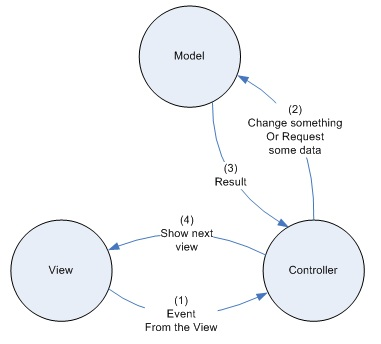
\includegraphics[width=0.5\linewidth]{images/mvc}
\caption{UML of the MVC architecture in our Map program}
\label{mvc-map}
\end{figure}

Figure \ref{mvc-map} shows our implementation of the MVC architecture. Because we 
have exactly one window, we chose to name our view and controller
``\class{View}'' and ``\class{Control}'', respectively. The same goes for the
models. We only have one data source (Krak's data-set), og because of that our model is called ``\class{Model}''. We
could have named these three classes something different that may have been more meaningful in
terms of the \class{Map of Denmark} context, but we chose these name in order to
make our architecture clear.

The easiest way to understand MVC and how the individual parts talk together, is by 
using an example. Let us say the user has already clicked the map and placed a
pin. Now the user clicks on the map again to place another pin.

The controller has placed listeners in the view, so when a MouseClicked event is
thrown, the controller is called. First it checks if there is another pin at the
spot of the click. If there is, this will be removed, and the model is told to
clear the route. If there is still over two pins placed, the model is asked to
calculate a new route.

If there isn't a pin where the user clicks, we place a new pin. If the user has
placed two or more pins, the controller calls its own findPath-method from point
1 to point 2, point 2 to point 3 and so on. The findPath()-method tells the
model to find a path between the two points given.

The model then asks a helper-class to find a path, using the A* algorithm, and
provides it with the graph and the two points. When a path is found, it is saved
in the model, ready for use in the controller.

The final step is getting the view to draw the route. The controller gets ready
for a repaint, by fetching the route from the model. Then it passes this route
to the view's repaint-method, and the view paints the road.

\section{Simple Diagram}
\label{UML-SD}

\section{Control flow}
\label{UML-CF}